Per l'esecuzione dell'esperienza è stato utilizzato il seguente apparato sperimentale:
\begin{itemize}
	\item Un calorimetro con coperchio munito di agitatore e foro per il termometro;
	\item Un fornellino;
	\item Un blocchetto di metallo;
	\item Un filo sottile di rame;
	\item Un becher;
	\item Acqua distillata;
	\item Pinze per becher;
	\item Bilancia digitale;
	\item Termometro digitale.
\end{itemize}

\begin{table}[H]
	\centering
	\begin{tabular}{|c|c|}
		\hline
		\textbf{Strumenti di misura} & \textbf{Risoluzione} \\
		\hline
		Bilancia digitale & $0.01\ g$ \\
		\hline
		Termometro digitale & $0.1^{\circ}C$ \\
		\hline
	\end{tabular}
	\caption{Risoluzione degli strumenti di misura utilizzati}
	\label{tab:}
\end{table}

\begin{figure}[H]
	\centering
	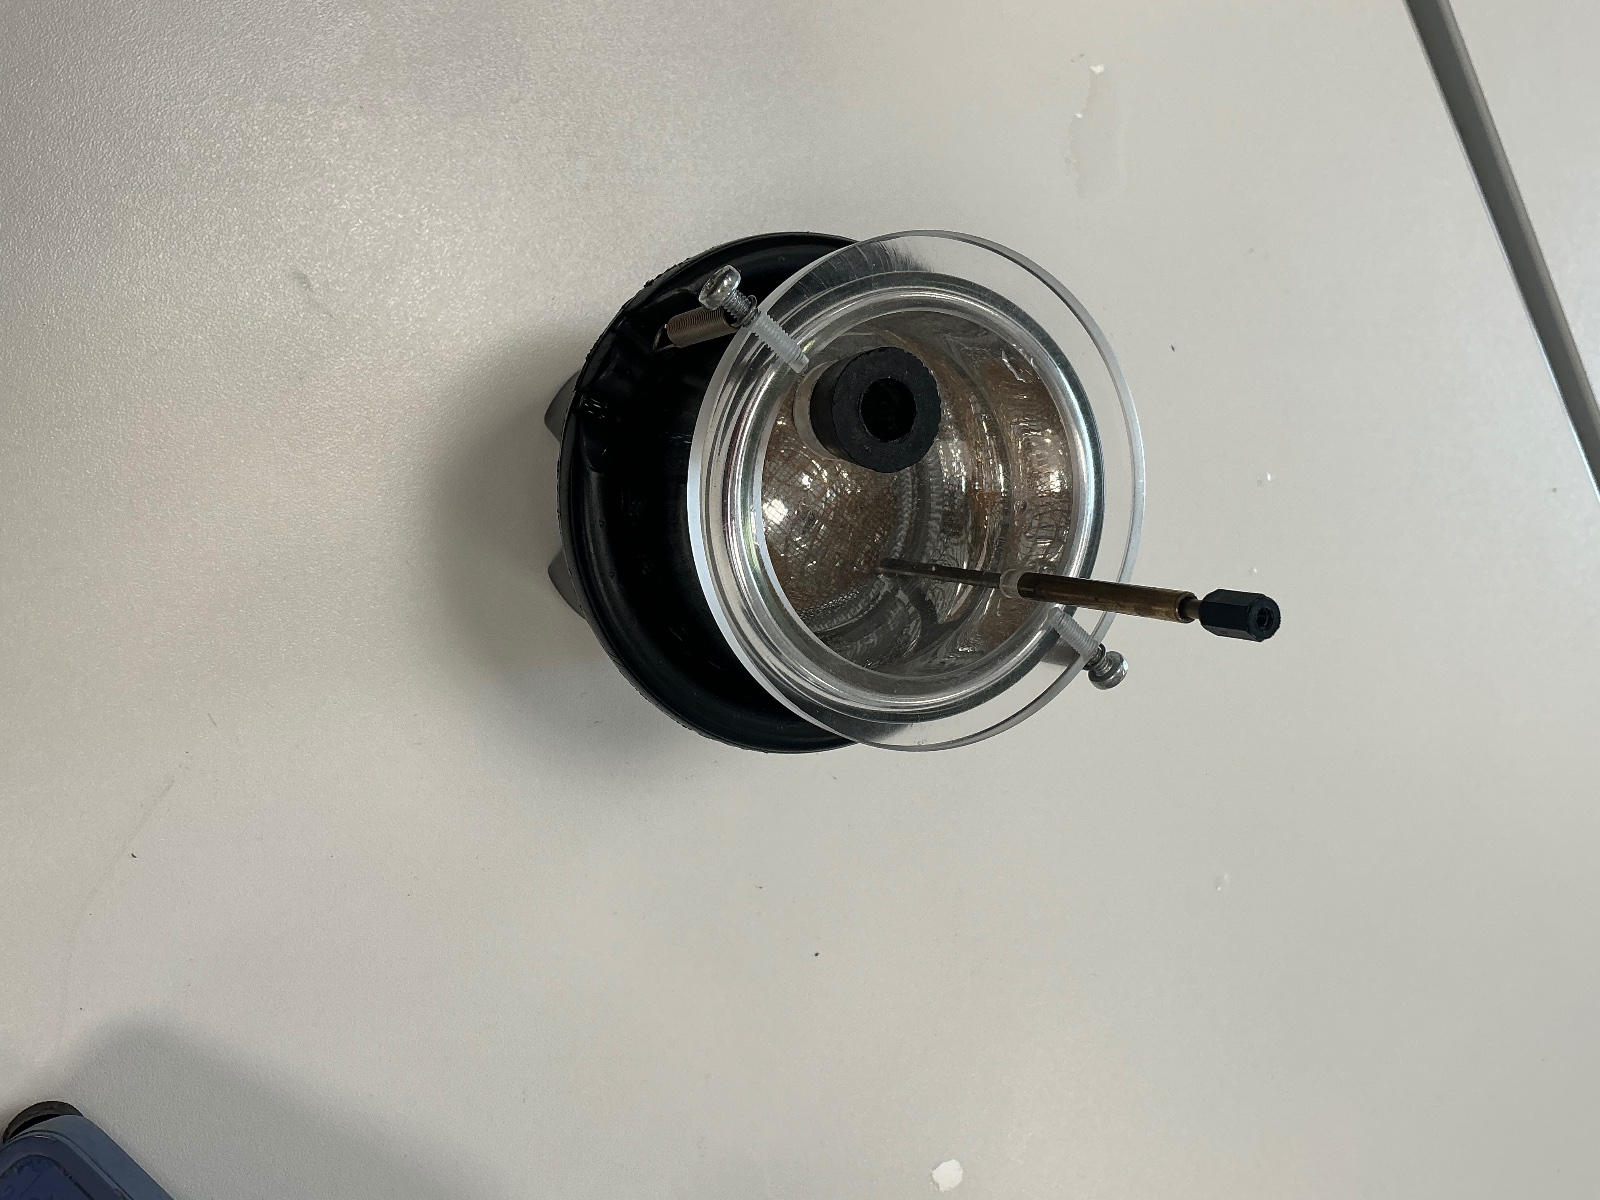
\includegraphics[width=0.55\textwidth]{./figures/calorimetro}
	\caption{Calorimetro utilizzato per l'esperimento.}
\end{figure}

\begin{figure}[H]
	\centering
	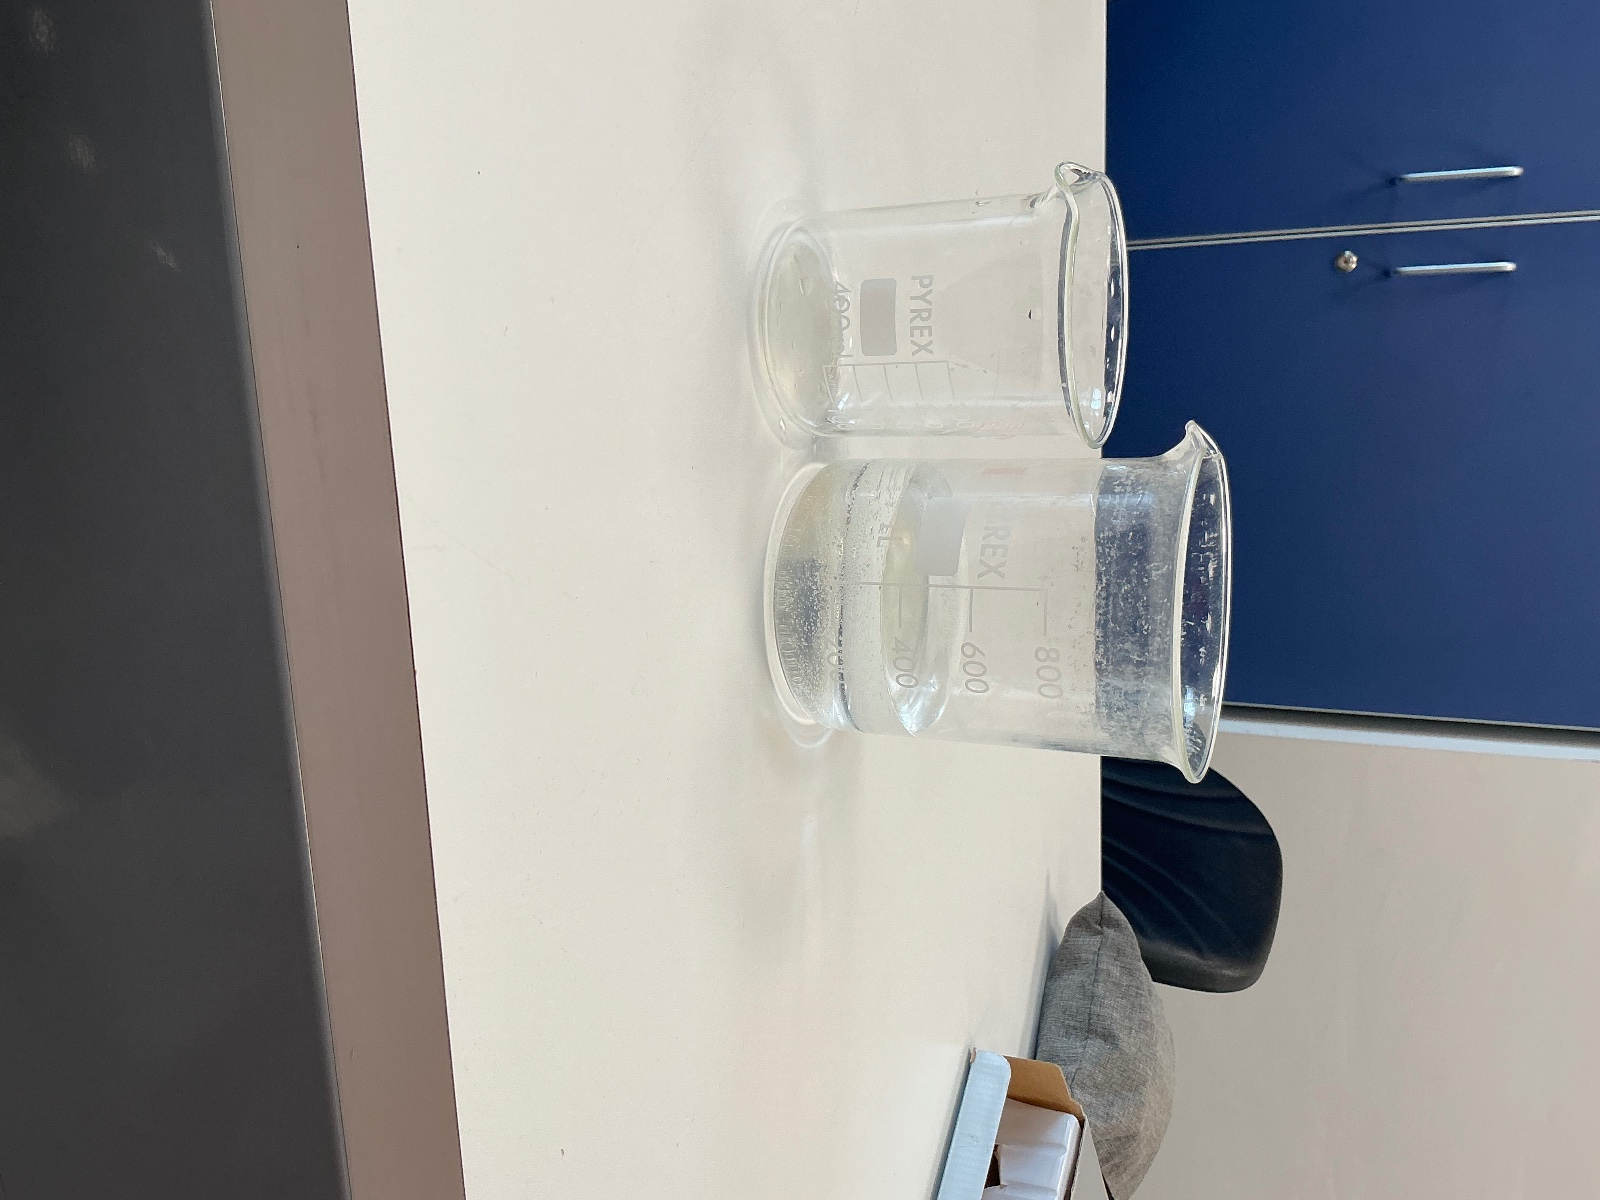
\includegraphics[width=0.55\textwidth]{./figures/becher}
	\caption{Becher utilizzati per l'esperimento.}
\end{figure}

\begin{figure}[H]
	\centering
	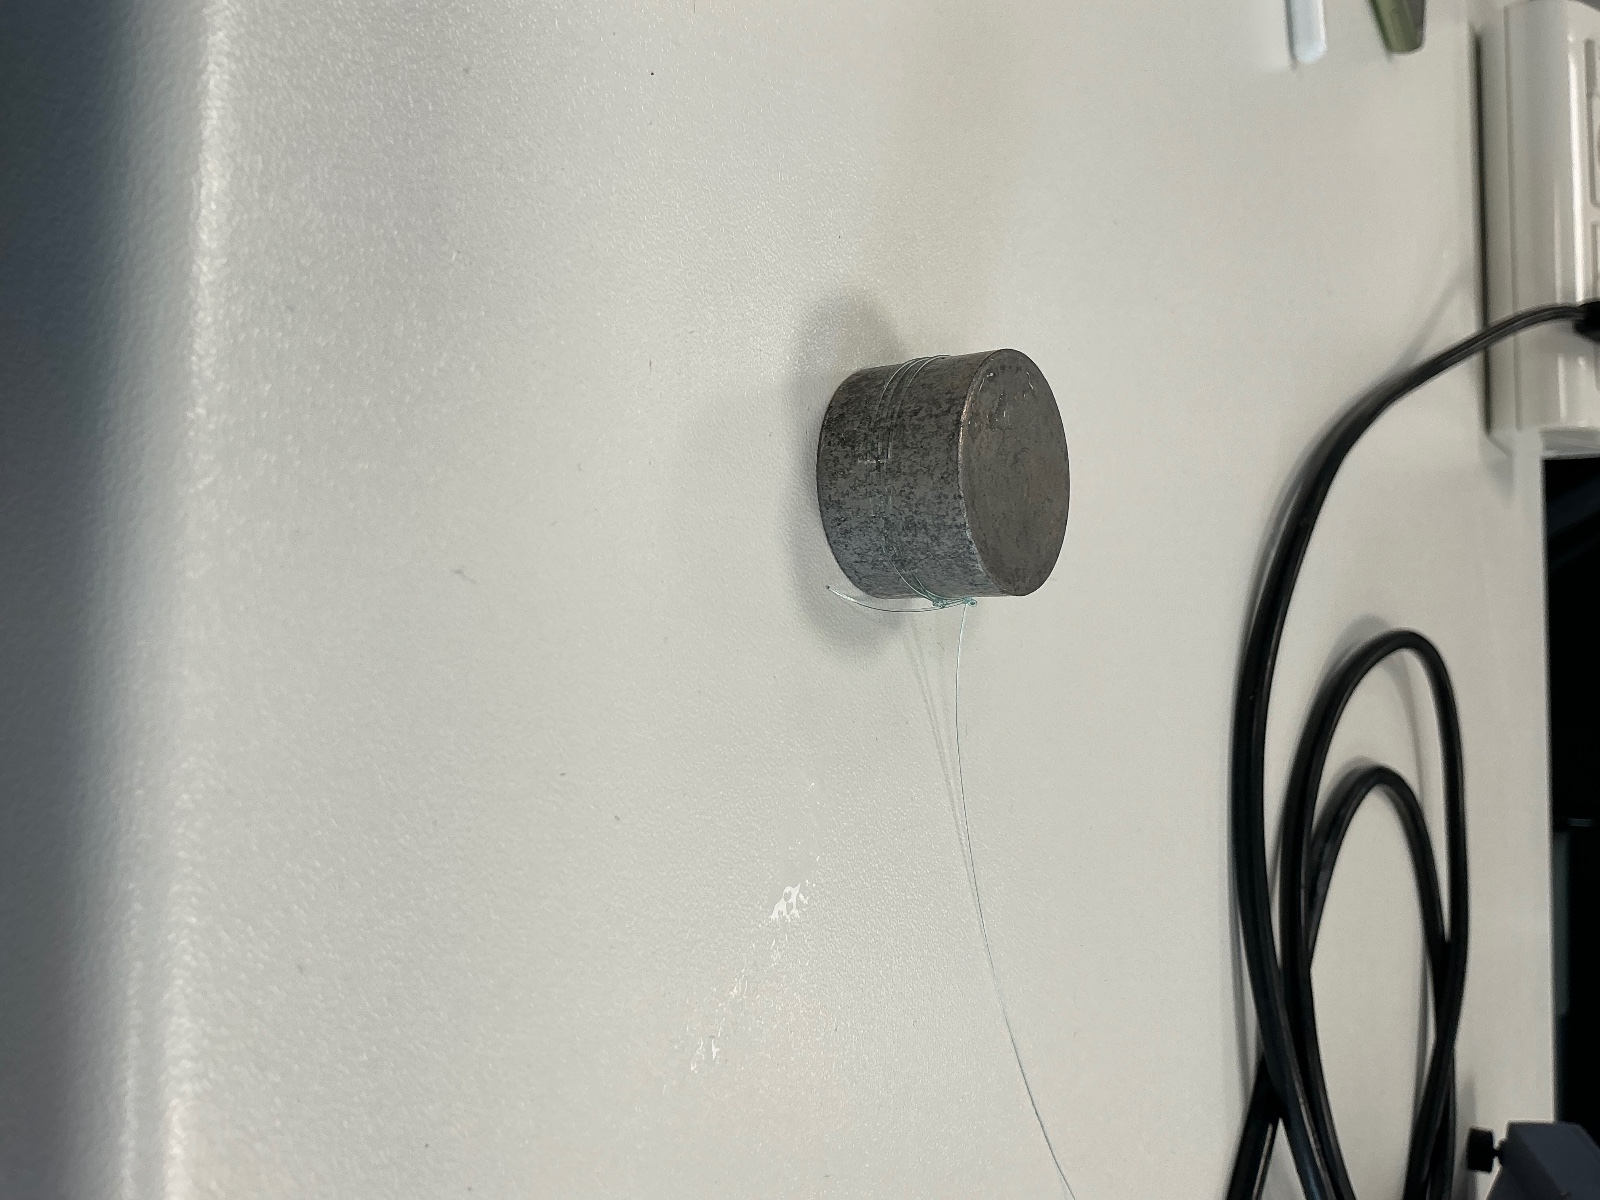
\includegraphics[width=0.55\textwidth]{./figures/materiale}
	\caption{Metallo utilizzato per l'esperimento e di cui è stato stimato il calore specifico.}
\end{figure}